\section{Results}

Each \Cyclus result is shown as a solid line, and the excel solution in the
paper is shown as a dotted line, for better visualization. The results are
simply a reproduction of the plots displayed in the paper. The excel
results are obtained by personal contact with the paper author
Bo Feng at Argonne National Laboratory.

Most results from \Cyclus show excellent agreement. Differences in results
stem from the errors associated with averaging and the concept of what
constitutes a `snapshot' of a facility inventory.

The deployed reactor capacity is shown in figure \ref{fig:pow_plot}.
The \gls{LWR} retirement and \gls{SFR} deployment timeseries are shown
in figure \ref{fig:dep}. The two plots show exact agreement with the
excel solutions from the paper.

\begin{figure}[htbp!]
	\begin{center}
		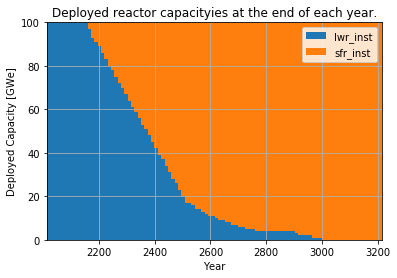
\includegraphics[scale=0.6]{./images/results_18/power_plot.png}
	\end{center}
        \caption{Deployed reactor capacities at the end of each year.}
	\label{fig:pow_plot}
\end{figure}



\begin{figure}[htbp!]
	\begin{center}
		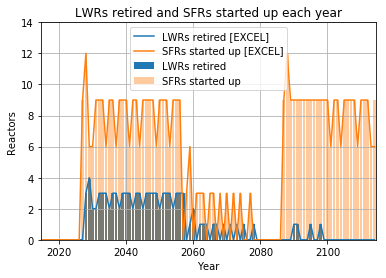
\includegraphics[scale=0.6]{./images/results_18/dep.png}
	\end{center}
        \caption{\glspl{LWR} retired and \glspl{SFR} started up each year.}
	\label{fig:dep}
\end{figure}


The annual fuel loading rates are shown in table \ref{fig:fuel_load}.
The initial fuel loading for 100 \gls{LWR} reactors were edited to match
the plot in the verification
study results. Note the oscillations for the \gls{LWR} fuel loading
is caused by the refueling period being 18-month refuel cycle for all \gls{LWR} reactors
aggregated into 12-month groups. Note also that the total values
are equal for both plots.

Although indistinguishable,
there is a small difference with \gls{SFR} fuel loading, that is proportional
to the core mass difference, as mentioned in the previous section.
Figure \ref{fig:fuel_load_diff_norm} shows the
differences normalized by the core mass differences, overlapped with the
\gls{SFR} deployment. This is to show that the differences only occur during
deployment due to the difference in core mass.


\begin{figure}[htbp!]
    \begin{center}
        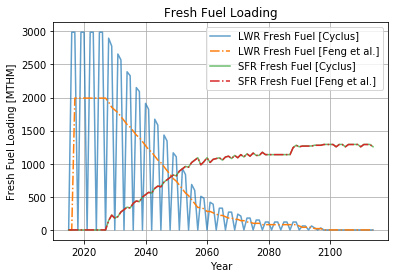
\includegraphics[scale=0.6]{./images/results_18/fuel_load.png}
    \end{center}
        \caption{Annual fresh fuel loading rates (first cores and reload fuel).}
    \label{fig:fuel_load}
\end{figure}


\begin{figure}[htbp!]
    \begin{center}
        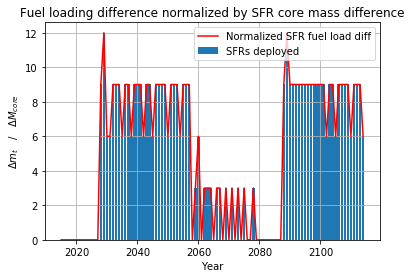
\includegraphics[scale=0.6]{./images/results_18/fuel_load_diff_norm.png}
    \end{center}
        \caption{Difference of annual fresh fuel loading rates (Cyclus - Excel) normalized by the core mass difference of an \gls{SFR} due to fractional batch size.}
    \label{fig:fuel_load_diff_norm}
\end{figure}


The inventory of discharged \gls{UNF} in mandatory cooling stage is shown
in figure \ref{fig:fuel_discharge}. It also oscillates between the excel solution,
and converges. This is due to the annual averaging of
the \gls{UNF} inventory. For a better visual, the monthly inventory is shown
in figure \ref{fig:fuel_discharge_monthly}, where the oscillation is more obvious.
Note that for most plots the \gls{SFR} inventory and fuel loading is almost
exactly the same as the excel solutions, minus the small difference due to core
size.

\begin{figure}[htbp!]
    \begin{center}
        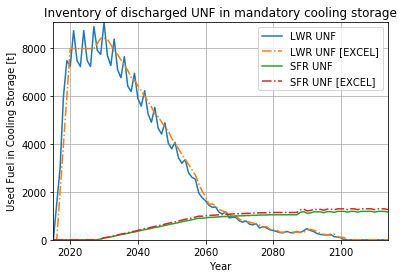
\includegraphics[scale=0.6]{./images/results_18/fuel_discharge.png}
    \end{center}
        \caption{Inventory of discharged \gls{UNF} in mandatory cooling storage.}
    \label{fig:fuel_discharge}
\end{figure}


\begin{figure}[htbp!]
    \begin{center}
        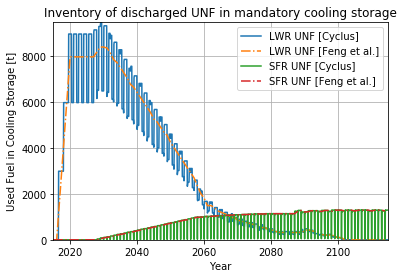
\includegraphics[scale=0.6]{./images/results_18/fuel_discharge_monthly.png}
    \end{center}
        \caption{Inventory of discharged \gls{UNF} in mandatory cooling storage.}
    \label{fig:fuel_discharge_monthly}
\end{figure}


Similar results are shown in figure \ref{fig:waiting} for the inventory of discharge fuel cooled and waiting
for reprocessing. Non-aggregated monthly values are shown in figure \ref{fig:waiting_monthly}.
However, note that the oscillation peaks meet with the excel
solution.  This is because cooled inventory is measured by the cumulative sum
of fuel that has been cooled minus the fuel reprocessed at that timestep.
The cooled inventory before the fuel are sent to reprocessing, which correspond
to the peaks in the oscillation, are the cooled inventory defined by the paper.

\begin{figure}[htbp!]
    \begin{center}
        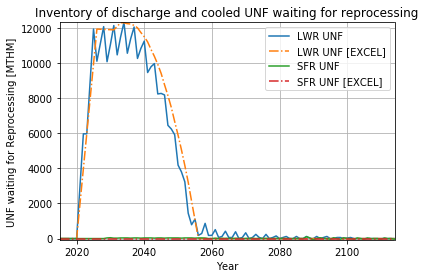
\includegraphics[scale=0.6]{./images/results_18/waiting.png}
    \end{center}
        \caption{Inventory of discharged and cooled \gls{UNF} waiting for reprocessing}
    \label{fig:waiting}
\end{figure}

\begin{figure}[htbp!]
    \begin{center}
        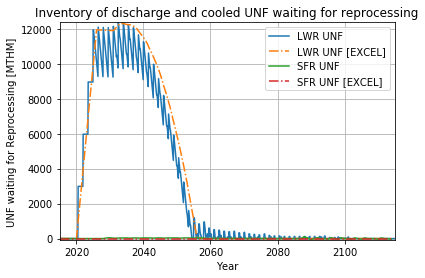
\includegraphics[scale=0.6]{./images/results_18/waiting_monthly.png}
    \end{center}
        \caption{Inventory of discharged and cooled \gls{UNF} waiting for reprocessing.}
    \label{fig:waiting_monthly}
\end{figure}


Figure \ref{fig:rep} shows the reprocessing throughput, which also oscillates between
the excel solution. Note that there is no oscillation in the beginning because the
\gls{LWR} reprocessing plant throughput is maximized at 2,000 tons per year. 

\begin{figure}[htbp!]
    \begin{center}
        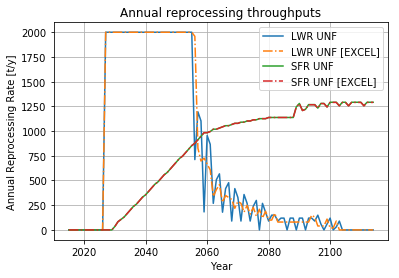
\includegraphics[scale=0.6]{./images/results_18/rep.png}
    \end{center}
        \caption{Annual reprocessing throughputs.}
    \label{fig:rep}
\end{figure}


Figure \ref{fig:tru} shows the inventory of unused \gls{TRU} recovered from \gls{UNF}.
The \Cyclus results follows the excel solutions closely. However, the difference
in core size causes \Cyclus results to be smaller, since more \gls{TRU} is used to
start up the newly deployed \glspl{SFR}. As the \glspl{SFR} \gls{UNF} is used to
create \gls{SFR} fuel, the difference is lessened.

\begin{figure}[htbp!]
	\begin{center}
		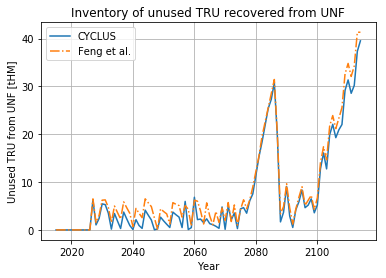
\includegraphics[scale=0.6]{./images/results_18/tru.png}
	\end{center}
        \caption{Inventory of unused \gls{TRU} recovered from \gls{UNF}.}
	\label{fig:tru}
\end{figure}

